\documentclass[12pt,a4paper]{article}
\usepackage{amsmath,amsthm,amsfonts,amssymb,amscd}
\usepackage{times}     
\usepackage{bookmark}         
\usepackage{graphicx}           
\usepackage{float}              
\usepackage{booktabs}           
\usepackage{xcolor}             
\usepackage{geometry}           
\usepackage{fullpage}           
\usepackage{comment}                     
\usepackage{listings}           
\usepackage{lastpage}           
\usepackage{fancyhdr}           
\usepackage{hyperref}           
\usepackage[small,bf]{caption}  
\usepackage{multicol}
\usepackage{tikz}               
\usepackage{circuitikz}         
\usepackage{verbatim}          
\usepackage{cite}               
\usepackage[us]{datetime} 
\usepackage{blindtext}
\usepackage[utf8]{vietnam}
\usepackage{array}
\usepackage{makecell}
\usepackage{tabularx}
\usepackage{titlesec}
\usepackage{enumitem}

\setlength\parindent{0pt}

%%%%%%%%%%%%%%%%%%%%%%%%%%%%%%%%%%%%%%%%%%%%%%%%%%%%%%%%%%%%%%
\titleformat{\section}
{\color{UM_DarkBlue}\normalfont\large\bfseries}
{\color{UM_DarkBlue}\thesection}{1em}{}

%%%%%%%%%%%%%%%%%%%%%%%%%%%%%%%%%%%%%%%%%%%%%%%%%%%%%%%%%%%%%%
\hypersetup{
    draft=false,
    final=true,
    colorlinks=true,
    citecolor=UM_DarkBlue,
    anchorcolor=yellow,
    linkcolor=UM_DarkBlue,
    urlcolor=UM_DarkBlue,
    filecolor=green,      
    pdfpagemode=FullScreen,
    bookmarksopen=false
    }
    
%%%%%%%%%%%%%%%%%%%%%%%%%%%%%%%%%%%%%%%%%%%%%%%%%%%%%%%%%%%%%%
\lstdefinestyle{Fortran}{
basicstyle=\scriptsize,        % the size of the fonts that are used for the code
  breakatwhitespace=false,         % sets if automatic breaks should only happen at whitespace
  breaklines=false,                 % sets automatic line breaking
  captionpos=b,                    % sets the caption-position to bottom
  commentstyle=\color{mygreen},    % comment style
  extendedchars=true,              % lets you use non-ASCII characters; for 8-bits encodings only, does not work with UTF-8
  keepspaces=true,                 % keeps spaces in text, useful for keeping indentation of code (possibly needs columns=flexible)
  keywordstyle=\color{blue},       % keyword style
  language=[95]Fortran,                 % the language of the code
  numbers=left,                    % where to put the line-numbers; possible values are (none, left, right)
  numbersep=5pt,                   % how far the line-numbers are from the code
  numberstyle=\tiny\color{mygray}, % the style that is used for the line-numbers
  rulecolor=\color{black},         % if not set, the frame-color may be changed on line-breaks within not-black text (e.g. comments (green here))
  showspaces=false,                % show spaces everywhere adding particular underscores; it overrides 'showstringspaces'
  showstringspaces=false,          % underline spaces within strings only
  showtabs=false,                  % show tabs within strings adding particular underscores
  stepnumber=1,                    % the step between two line-numbers. If it's 1, each line will be numbered
  stringstyle=\color{mymauve},     % string literal style
  tabsize=4,                       % sets default tabsize to 2 spaces
  title=\lstname                   % show the filename of files
}

%%%%%%%%%%%%%%%%%%%%%%%%%%%%%%%%%%%%%%%%%%%%%%%%%%%%%%%%%%%%%%%
\definecolor{UM_Brown}{HTML}{3D190D}
\definecolor{UM_DarkBlue}{HTML}{2264B0}
\definecolor{UM_LightBlue}{HTML}{1CA9E1}
\definecolor{UM_Orange}{HTML}{fEB415}




%\newcommand{\tu}[1]{\textup{#1}}
\newcommand{\tu}[1]{\mathrm{#1}}







\newcommand{\ones}{\mathbf 1}
\newcommand{\reals}{{\mbox{\bf R}}}
\newcommand{\integers}{{\mbox{\bf Z}}}
\newcommand{\symm}{{\mbox{\bf S}}}  % symmetric matrices

\newcommand{\nullspace}{{\mathcal N}}
\newcommand{\range}{{\mathcal R}}
\newcommand{\Rank}{\mathop{\bf Rank}}
\newcommand{\Tr}{\mathop{\bf Tr}}
\newcommand{\diag}{\mathop{\bf diag}}
\newcommand{\card}{\mathop{\bf card}}
\newcommand{\rank}{\mathop{\bf rank}}
\newcommand{\conv}{\mathop{\bf conv}}
\newcommand{\prox}{\mathbf{prox}}

\newcommand{\Expect}{\mathop{\bf E{}}}
\newcommand{\Prob}{\mathop{\bf Prob}}
\newcommand{\Co}{{\mathop {\bf Co}}} % convex hull
\newcommand{\dist}{\mathop{\bf dist{}}}
\newcommand{\argmin}{\mathop{\rm argmin}}
\newcommand{\argmax}{\mathop{\rm argmax}}
\newcommand{\epi}{\mathop{\bf epi}} % epigraph
\newcommand{\Vol}{\mathop{\bf vol}}
\newcommand{\dom}{\mathop{\bf dom}} % domain
\newcommand{\intr}{\mathop{\bf int}}
\newcommand{\sign}{\mathop{\bf sign}}

\newcommand{\cf}{{\it cf.}}
\newcommand{\eg}{{\it e.g.}}
\newcommand{\ie}{{\it i.e.}}
\newcommand{\etc}{{\it etc.}}

\graphicspath{{Figs/}}

\begin{document}

\textcolor{UM_Brown}{
\begin{minipage}{0.1\textwidth}
    \begin{flushleft}
        \includegraphics[height=3.5cm]{logo.eps}
    \end{flushleft}
\end{minipage}
\begin{minipage}{0.8\textwidth}
    \begin{center}
        \textbf{\Large Nhập môn mạng máy tính}\\
        \vspace{5pt}
        Assignment 5 \\
        \vspace{10pt}
        \textit{Group 9 - FOBE} \\
        \vspace{5pt}
        \longdate\today
    \end{center}
\end{minipage}
\vspace{10pt}
\hrule
}

\section*{Problem 23: Maximum sender window size given sequence number space k for each protocol}
\subsection*{1.\;GBN Protocol}
\begin{itemize}
    \item Nếu \textit{window sender size} đúng bằng \textbf{k} và trong trường hợp toàn bộ ACKs bị mất. Window receiver đã di chuyển (do bên nhận không thể biết được nếu ACKs bị mất) trong
khi window sender vẫn giữ nguyên và gửi lại các packet cũ. Bên nhận không cách nào phân biệt được gói tin mới và cũ;
    \item Do đó \textit{window sender size} $\le$ k - 1.
\end{itemize}

\subsection*{2.\; SR Protocol}
\begin{itemize}
    \item Giống như GBN Protocol, ta cần tránh trường hợp chồng chéo gói tin giữa gói tin có sequence number cao nhất ở sender window với gói
tin có sequence number có sequence number nhỏ nhất ở receiver window \textbf{ở bất kì thời điểm nào}.
    \item Giả sử sequence number nhỏ nhất mà bên nhận đang đợi packet là \textit{s}. Lúc này cửa sổ bên nhận là [s, s + w - 1] trong đó w là kích thước cửa số. Và trong trường
hợp các ACKs của các gói tin trước đó đều bị mất nghĩa là cửa sổ bên gửi hiện tại đang là [s-w, s-1].
    \item Để tránh hiện tượng chồng chéo thì \textbf{k} tức kích thước của sequece number phải bao đủ cả sender window và receiver window. Do đó k > (s-w) + (s+w-1) $\Rightarrow$ k $\ge$ 2w
    \item Vậy window sender size $\le$ $\frac{k}{2}$
\end{itemize}

\begin{figure}[h]
    \centering
    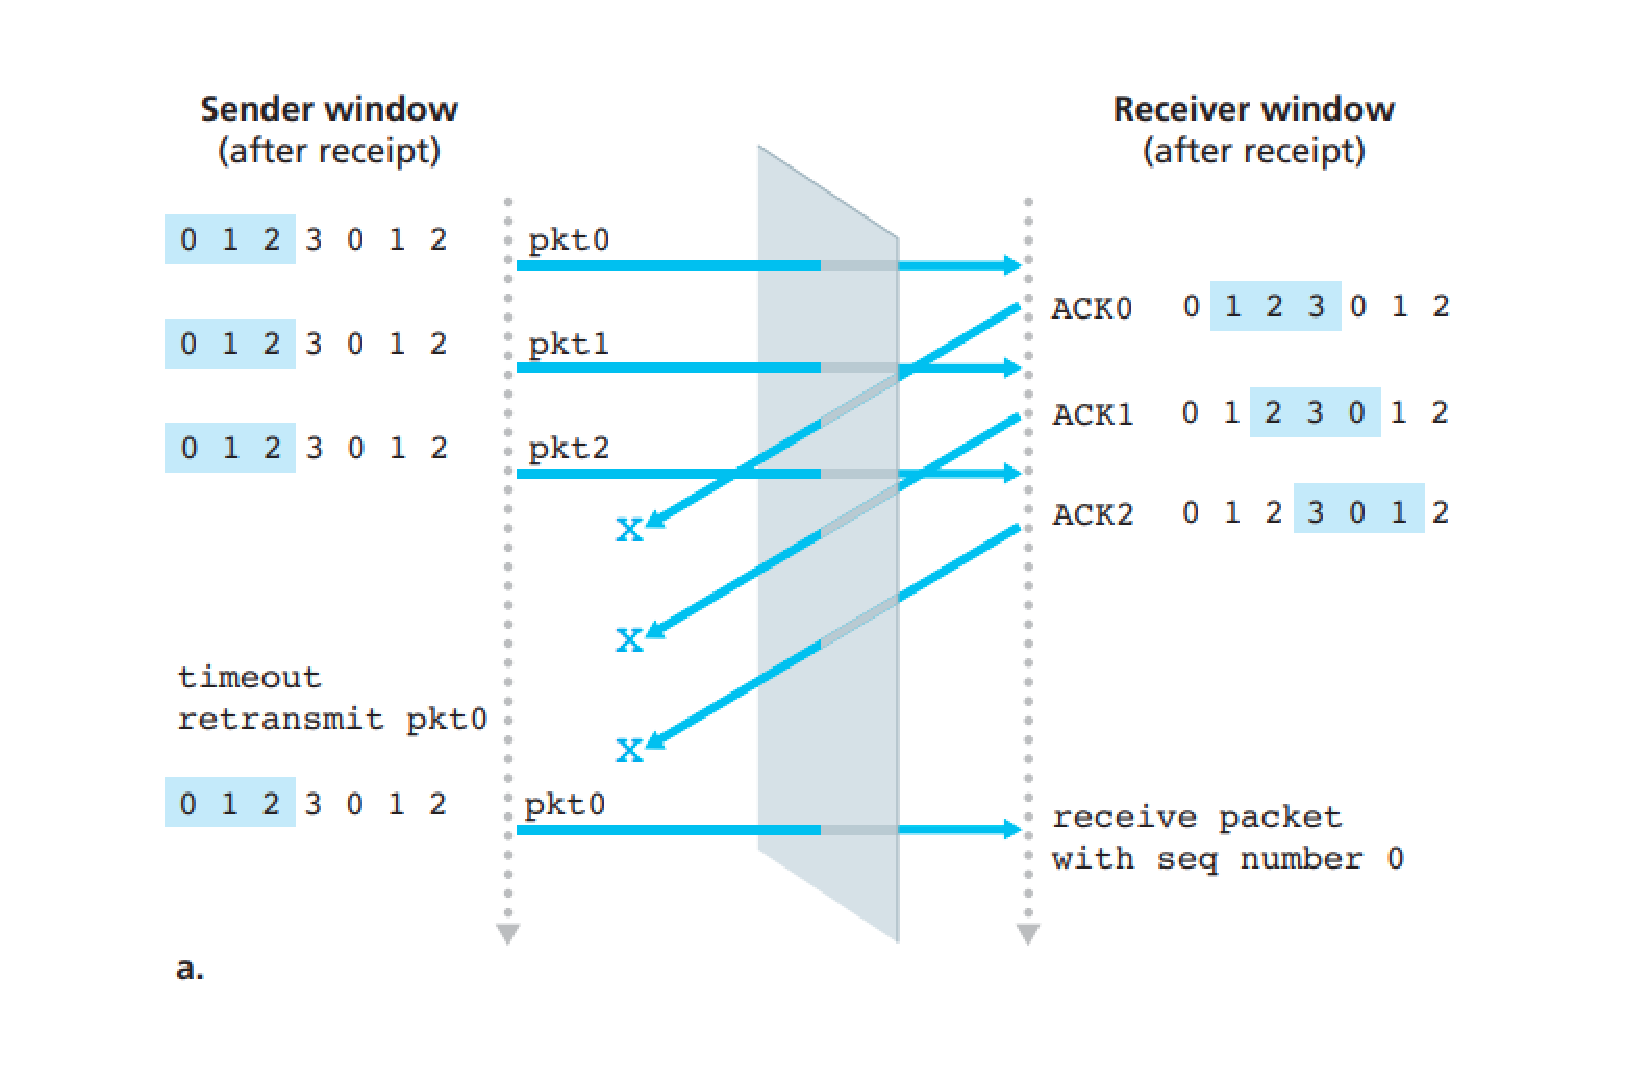
\includegraphics[scale=0.29]{f327a.eps}
    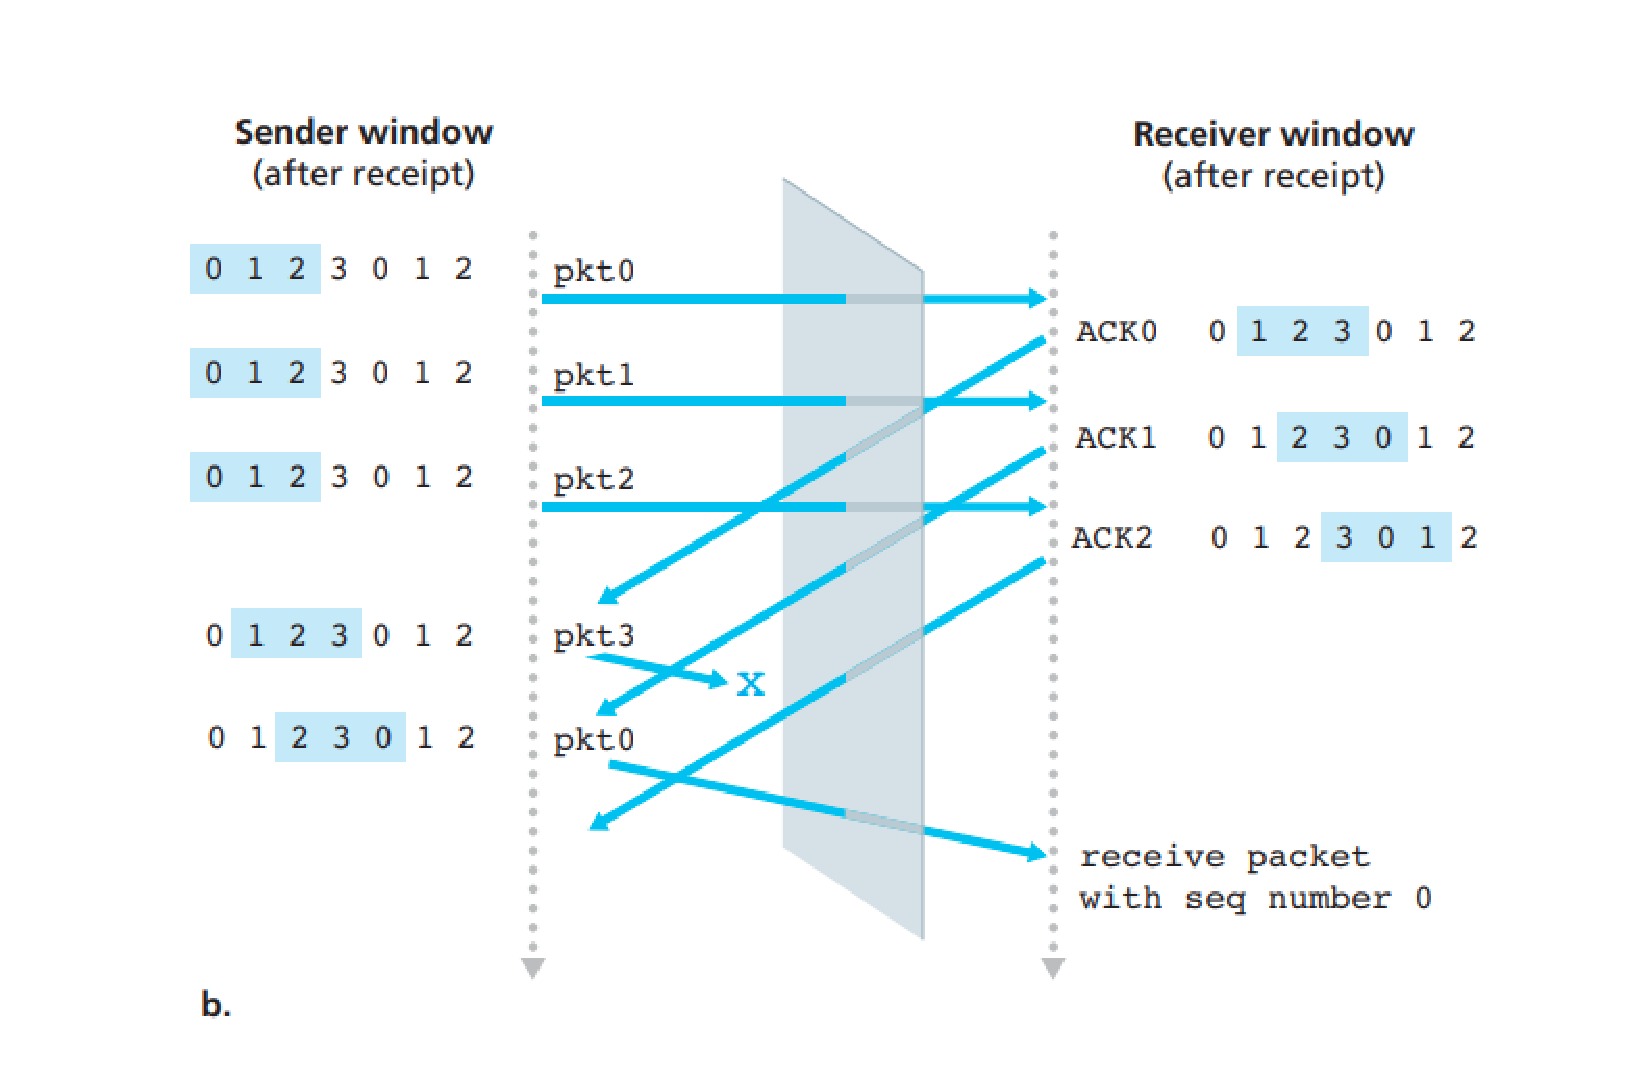
\includegraphics[scale=0.29]{f327b.eps}
\end{figure}

\newpage
\section*{Problem 24: True or False}


\begin{description}[font=$\bullet$~\normalfont\scshape\color{red!50!black}]
    \item [A True] Đối với SRP, bên gửi có thể nhận các ACKs nằm ngoài cửa sổ hiện tại
\end{description}
Giả sử Bên gửi gửi các gói tin, bên nhận nhận được rồi trả về các ACKs, tuy nhiên do time out nên bên gửi lại các gói tin trên, bên nhận được
các bản sao và gửi lại ACKs, bên gửi nhận được ACKs và tăng cửa sổ lên. Lúc này ACKs lúc trước đã đến và nó nằm ngoài cửa sổ hiện tại.

\begin{description}[font=$\bullet$~\normalfont\scshape\color{red!50!black}]
    \item [B True] Đối với GBN, bên gửi có thể nhận ACK nằm ngoài cửa sổ hiện tại
\end{description}
Tương tự như với SRP, ta chỉ thay các individual ack thành một cumulative ack.


\begin{description}[font=$\bullet$~\normalfont\scshape\color{red!50!black}]
    \item [C True] ABP tương tự như SRP khi window sender size = window receiver size = 1
\end{description}
SRP có thể xem như ABP với kích thước cửa sổ W. \\
Nói cách khác khi W = 1, SRP là ABP.
\begin{description}[font=$\bullet$~\normalfont\scshape\color{red!50!black}]
    \item [D True] ABP tương tự như GBN khi window sender size = 1
\end{description}
ABP cũng có thể được xem như một trường hợp đặt biệt của GBN khi \textit{window sender size} = 1


\section*{Problem 27}
\subsection*{A. In the second segment sent from Host A to B}
\begin{itemize}
    \item \textit{Sequence number = 127 + 80 = 207}
    \item \textit{Source port number = 302}
    \item \textit{Destination port number = 80}
\end{itemize}

\subsection*{B. If the first segment arrives before the second segment, in the acknowledgement of the first arriving segment}
\begin{itemize}
    \item Acknowledgement number = 207
    \item Source port number = 80
    \item Destination port number = 302
\end{itemize}

\subsection*{C. If the second segment arrives before the first segment, in the acknowledgement of the first arriving segment}
\begin{itemize}
    \item Acknowledgement number = 127
\end{itemize}

\newpage
\subsection*{D. Timing diagram}
\begin{figure}[h]
    \centering
    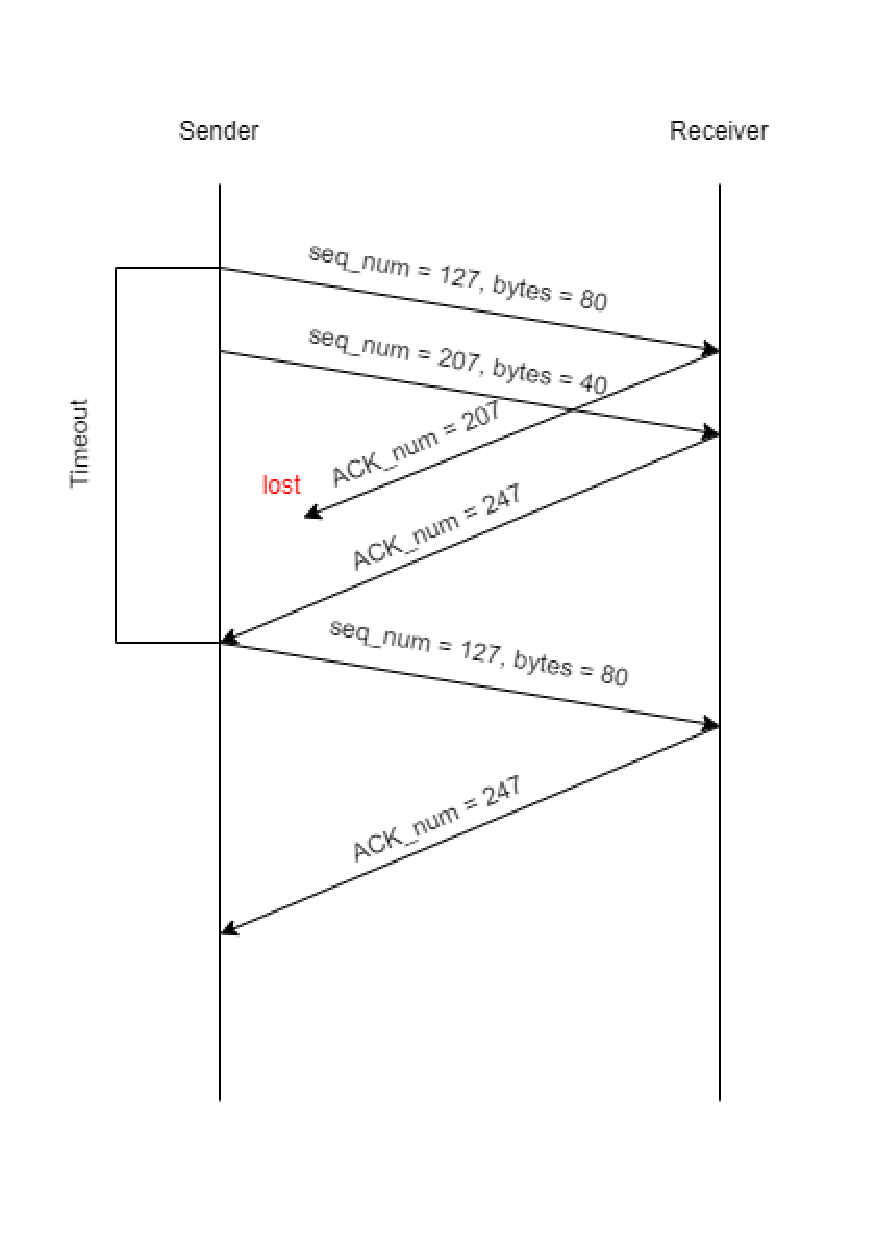
\includegraphics[scale=0.5]{P27_d.drawio.eps}
\end{figure}


\section*{P28: ANS - Effect of TCP flow control}
\begin{itemize}
    \item  As given that the link capacity is only 100 Mbps, so the sending rate of Host A can be almost 100 Mbps;
    \item  Host A sends data into the TCP receive buffer at a rate as high as 120 Mbps;
    \item The receive buffer fills up at a rate of about 50Mbps;
    \item Host B removes data from the TCP receive buffer at a rate of 50 Mbps;
    \item When the TCP receive buffer is full, Host B sets the RcvWindow to 0. It is a signal to Host A to stop sending data;
    \item  Host A stops sending the data into TCP receive buffer and waits till it receives a TCP segment with RcvWindow > 0;
    \item Host A will stop and start sending data depending on the value of the RcvWindow that Host A receives from Host B;
    \item Thus it can be determined that the on an average, the long-term rate at which Host A sends data to Host B can be no more than 50Mbps.
\end{itemize}

\section*{P30}
Calculate the EstimatedRTT after obtaining the first sample RTT=106ms:
\begin{equation*}
    \begin{split}
        EstimatedRTT &= a * SampleRTT+(1- a) * EstimatedRTT \\
                     &= 0.125 * 106 + (1-0.125) * 100 \\
                     &= 13,25 + 87.5 \\
                     &= 100.75 \; ms \\
    \end{split}
\end{equation*}
Calculate the DevRTT after obtaining the first sample RTT:
\begin{equation*}
    \begin{split}
        DevRTT &= \beta * | SampleRTT- EstimatedRTT|+(1- \beta )* DevRTT \\
                     &= 0.25 * |106-100.75| + (1-0.25) *5 \\
                     &= 1.3125 + 3.75 \\
                     &= 5.062 \; ms \\
    \end{split}
\end{equation*}
Calculate the Timeout Interval after obtaining the first sample RTT:
\begin{equation*}
    \begin{split}
        TimeoutInterval &= EstimatedRTT +4* DevRTT \\
                     &= 100.75 + 4 *5.0625 \\
                     &= 121 \; ms\\
    \end{split}
\end{equation*}

Calculate the EstimatedRTT after obtaining the second sample RTT=120ms:
\begin{equation*}
    \begin{split}
        EstimatedRTT &= a * SampleRTT+(1- a) * EstimatedRTT \\
                     &= 0.125 * 120 + (1-0.125) * 100.75 \\
                     &= 15 + 88.15625\\
                     &= 103.15625 \; ms \\
    \end{split}
\end{equation*}
Calculate the DevRTT after obtaining the second sample RTT:
\begin{equation*}
    \begin{split}
        DevRTT &= \beta * | SampleRTT- EstimatedRTT|+(1- \beta )* DevRTT \\
                     &= 0.25 * |120-103.15625| + (1-0.25) *5.0625 \\
                     &= 4.21 + 3.79 \\
                     &= 8 \; ms \\
    \end{split}
\end{equation*}
Calculate the Timeout Interval after obtaining the second sample RTT:
\begin{equation*}
    \begin{split}
        TimeoutInterval &= EstimatedRTT +4* DevRTT \\
                     &= 103.15625 + 4 *8\\
                     &= 135.15 \; ms\\
    \end{split}
\end{equation*}

Calculate the EstimatedRTT after obtaining the second sample RTT=120ms:
\begin{equation*}
    \begin{split}
        EstimatedRTT &= a * SampleRTT+(1- a) * EstimatedRTT \\
                     &= 0.125 * 120 + (1-0.125) * 100.75 \\
                     &= 15 + 88.15625\\
                     &= 103.15625 \; ms \\
    \end{split}
\end{equation*}
Calculate the DevRTT after obtaining the second sample RTT:
\begin{equation*}
    \begin{split}
        DevRTT &= \beta * | SampleRTT- EstimatedRTT|+(1- \beta )* DevRTT \\
                     &= 0.25 * |120-103.15625| + (1-0.25) *5.0625 \\
                     &= 4.21 + 3.79 \\
                     &= 8 \; ms \\
    \end{split}
\end{equation*}
Calculate the Timeout Interval after obtaining the second sample RTT:
\begin{equation*}
    \begin{split}
        TimeoutInterval &= EstimatedRTT +4* DevRTT \\
                     &= 103.15625 + 4 *8\\
                     &= 135.15 \; ms\\
    \end{split}
\end{equation*}

Calculate the Timeout Interval after obtaining the second sample RTT:
\begin{equation*}
    \begin{split}
        TimeoutInterval &= EstimatedRTT +4* DevRTT \\
                     &= 103.15625 + 4 *8\\
                     &= 135.15 \; ms\\
    \end{split}
\end{equation*}

Calculate the EstimatedRTT after obtaining the third sample RTT=140ms:
\begin{equation*}
    \begin{split}
        EstimatedRTT &= a * SampleRTT+(1- a) * EstimatedRTT \\
                     &= 0.125 * 140 + (1-0.125) * 103.15 \\
                     &= 17.5 + 90.26\\
                     &= 107.75 \; ms \\
    \end{split}
\end{equation*}
Calculate the DevRTT after obtaining the third sample RTT:
\begin{equation*}
    \begin{split}
        DevRTT &= \beta * | SampleRTT- EstimatedRTT|+(1- \beta )* DevRTT \\
                     &= 0.25 * |140-107.75| + (1-0.25) *8 \\
                     &= 8.06 + 6 \\
                     &= 14.06 \; ms \\
    \end{split}
\end{equation*}
Calculate the Timeout Interval after obtaining the third sample RTT:
\begin{equation*}
    \begin{split}
        TimeoutInterval &= EstimatedRTT +4* DevRTT \\
                     &= 107.75 + 4 *14.06\\
                     &= 164 \; ms\\
    \end{split}
\end{equation*}

Calculate the Timeout Interval after obtaining the second sample RTT:
\begin{equation*}
    \begin{split}
        TimeoutInterval &= EstimatedRTT +4* DevRTT \\
                     &= 103.15625 + 4 *8\\
                     &= 135.15 \; ms\\
    \end{split}
\end{equation*}

Calculate the EstimatedRTT after obtaining the fourth sample RTT=90ms:
\begin{equation*}
    \begin{split}
        EstimatedRTT &= a * SampleRTT+(1- a) * EstimatedRTT \\
                     &= 0.125 * 90 + (1-0.125) * 107.75 \\
                     &= 11.25 + 94.28\\
                     &= 105.53 \; ms \\
    \end{split}
\end{equation*}
Calculate the DevRTT after obtaining the fourth sample RTT:
\begin{equation*}
    \begin{split}
        DevRTT &= \beta * | SampleRTT- EstimatedRTT|+(1- \beta )* DevRTT \\
                     &= 0.25 * |90-105.53| + (1-0.25) *14.06 \\
                     &= 3.88 + 10.545 \\
                     &= 14.42 \; ms \\
    \end{split}
\end{equation*}
Calculate the Timeout Interval after obtaining the fourth sample RTT:
\begin{equation*}
    \begin{split}
        TimeoutInterval &= EstimatedRTT +4* DevRTT \\
                     &= 105.53 + 4 *14.42\\
                     &= 163.21 \; ms\\
    \end{split}
\end{equation*}

Calculate the Timeout Interval after obtaining the second sample RTT:
\begin{equation*}
    \begin{split}
        TimeoutInterval &= EstimatedRTT +4* DevRTT \\
                     &= 103.15625 + 4 *8\\
                     &= 135.15 \; ms\\
    \end{split}
\end{equation*}

Calculate the EstimatedRTT after obtaining the fifth sample RTT=115ms:
\begin{equation*}
    \begin{split}
        EstimatedRTT &= a * SampleRTT+(1- a) * EstimatedRTT \\
                     &= 0.125 * 115 + (1-0.125) * 105.53 \\
                     &= 14.375 + 92.34\\
                     &= 106.715 \; ms \\
    \end{split}
\end{equation*}
Calculate the DevRTT after obtaining the fifth sample RTT:
\begin{equation*}
    \begin{split}
        DevRTT &= \beta * | SampleRTT- EstimatedRTT|+(1- \beta )* DevRTT \\
                     &= 0.25 * |115-106.715| + (1-0.25) *14.42 \\
                     &= 2.07 + 10.815 \\
                     &= 12.885 \; ms \\
    \end{split}
\end{equation*}
Calculate the Timeout Interval after obtaining the fifth sample RTT:
\begin{equation*}
    \begin{split}
        TimeoutInterval &= EstimatedRTT +4* DevRTT \\
                     &= 106.715 + 4 *12.885\\
                     &= 158.225 \; ms\\
    \end{split}
\end{equation*}


\section*{Contributors and Reference}
\begin{table}[H]
    \caption{Contributors}
    \centering
    \begin{tabular}{c|c}
    \toprule
     \bf{Problem }  & \textbf{Contributors} \\
     \midrule
     23 & Hoàng Tân \\
     24 & Trâm Anh \\
     27 & Kim Yến \\
     28, 31 & Gia Khang \\
     \bottomrule
    \end{tabular}
\end{table}

\url{http://www.cs.tau.ac.il/~allonwag/comnet2012A/Recitations/Comnet_Recitation7.pdf} \\
\url{https://studylib.net/doc/18365657/solution-link} \\


\end{document} 